\documentclass[text07.tex]{subfiles}
\begin{document}
% \refstepcounter{PagePtr}\label{P:HP}
% \refstepcounter{Exercise}

%
% subsection 6.3.2
%
\subsection{自分のホームページを公開しよう\label{E:myHP}}
% \subsection{2−2　\theExercise　自分のホームページを公開しよう\label{E:myHP}}
% \subsection*{2−2自分のホームページを公開しよう}
{\bfseries 考え方}


クライアントとサーバと呼ばれるコンピュータがあります。クライアントとはサービスを利用するコンピュータです。サーバとはそれと\ruby{逆}{ぎゃく}にサービスを提供しているコンピュータです。クライアントとサーバは同じコンピュータにあっても
OK です。例えば、Googleは検索するためのウェブサイトを提供しています。ウェブサイトを提供するサーバをウェブサーバと呼びます。自分のホームページを公開するためには、ウェブサーバを動かす必要があります。

注意

今回のみんなのホームページはローカルIPの間だけです。つまり、インターネット上に公開はしません。これを公開して、実際確認したりみんなで見せ合いをしてみましょう。


\bigskip

\begin{enumerate}
    \item まず
    {\textasciitilde}/06/wwwのディレクトリに移りましょう。

    ターミナルを立ち上げて次のコマンドを打ちましょう。

    cd {\textasciitilde}/06/www

    \item サーバを動かしてみましょう。

    次のコマンドを打ちましょう。

    ./webserver.py

    を実行するとウェブサーバが動き始めます。

    webserver.pyを起動したディレクトリがドキュメントルートになります。

    これはファイルシステムのルートディレクトリとは別のものでドキュメントルートはウェブ

    サーバから見たルートディレクトリのことです。

    つまりウェブサーバしかそのディレクトリをルートディレクトリとは認識しません。

    ディレクトリに関しては第3回の教科書3.3.2 「ディレクトリの関係」を参考にしてください。

    \begin{center}
        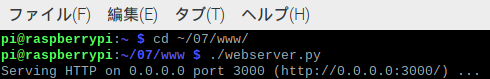
\includegraphics[width=0.73\textwidth]{../../asset/image/ome7-img038.png}
    \end{center}

    \item サーバが動いているかどうかを確認してみましょう。

    別のターミナルを立ち上げ、次のコマンドを打ちましょう。

    nmap localhost

    今回使っているポート番号は:3000です。STATE（状態）がopen（開く）になっています。

    これでサーバが動いていることが分かります。

    \begin{center}
        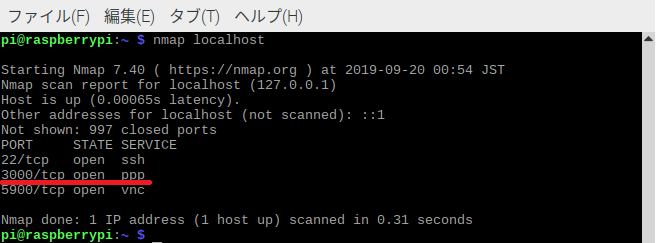
\includegraphics[width=0.75\textwidth]{../../asset/image/ome7-img039.png}
    \end{center}

    \clearpage

    \item みなさんが作ったウェブページを表示してみましょう。

    みなさんが作ったindex.htmlの場所はwebserver.pyを起動したディレクトリと同じでしたね。「2」で説明したドキュメントルートです。

    これはwebserver.pyを起動したディレクトリ

    {\textasciitilde}/06/www/

    を指しています。

    \bigskip

    次にブラウザのアドレスバーに打つURLはどのように書けばいいのでしょうか。

    URLの書き方は次のようになります。

    なので自分のパソコンのサーバを見るには

    \begin{center}
        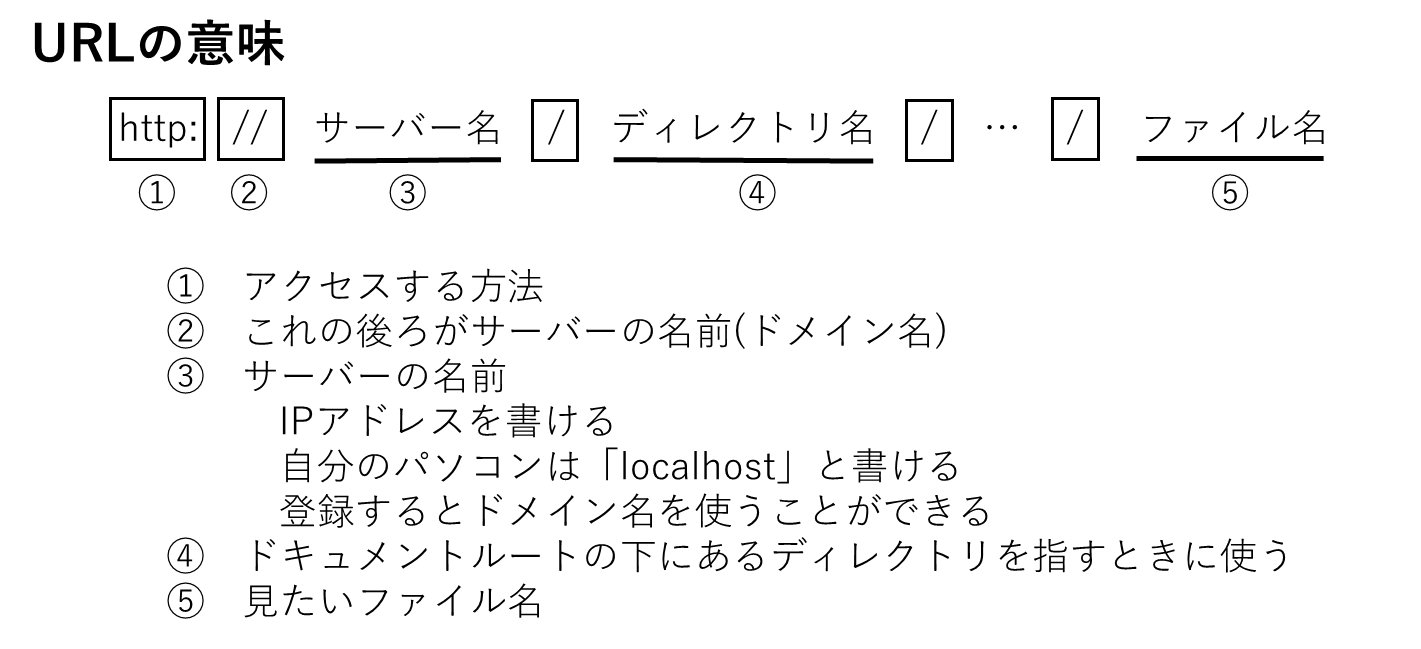
\includegraphics[width=13.894cm]{../../asset/image/ome7-img040.png}
    \end{center}

    \url{http://localhost:3000/}

    というURLになります。

    サーバ名の後の/（スラッシュ）はドキュメントルートを示しています。

    サーバはファイル名を指定しないとindex.htmlというファイルを開くように\ruby{設定}{せってい}されて\ \ います。

    \url{http://localhost:3000/}

    をブラウザのアドレスバーに打ってみましょう。

    みなさんが作ったウェブページのHTMLが表示されましたね。

    これは

    \url{http://localhost:3000/index.html}

    と入力しているのと同じことです。

    \bigskip
    \begin{center}
        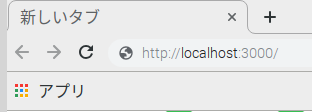
\includegraphics[width=9.551cm]{../../asset/image/ome7-img041.png}
    \end{center}

\end{enumerate}

\clearpage


% 1.まず
% {\textasciitilde}/07/wwwのディレクトリに移りましょう。

% \ \ ターミナルを立ち上げて次のコマンドを打ちましょう。

% \ \ cd {\textasciitilde}/07/www


% \bigskip

% 2.サーバーを動かしてみましょう。

% \ \ 次のコマンドを打ちましょう。

% \ \ 　./webserver.py

% \ \ を実行するとウェブサーバが動き始めます。

% \ \ webserver.pyを起動したディレクトリがドキュメントルートになります。

% \ \ これはファイルシステムのルートディレクトリとは別のものでドキュメントルートはウェブ

% \ \ サーバから見たルートディレクトリのことです。

% \ \ つまりウェブサーバーしかそのディレクトリをルートディレクトリとは認識しません。

% \ \ ディレクトリに関しては第3回の教科書3.3.2 「ディレクトリの関係」を参考にしてください。


% \centering
% 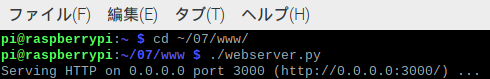
\includegraphics[width=0.73\textwidth]{../../asset/image/ome7-img038.png}
% \flushleft

% 3.サーバーが動いているかどうかを確認してみましょう。

% \ \ 別のターミナルを立ち上げ、次のコマンドを打ちましょう。

% \ \ 　nmap localhost

% \ \ 今回使っているポート番号は:3000です。STATE（状態）がopen（開く）になっています。

% \ \ これでサーバーが動いていることが分かります。

% \centering
% 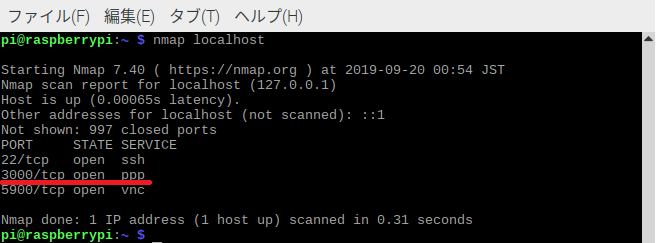
\includegraphics[width=0.75\textwidth]{../../asset/image/ome7-img039.png}
% \flushleft

% \clearpage


% 4.みなさんが作ったウェブページを表示してみましょう。

% \ \ みなさんが作ったindex.htmlの場所はwebserver.pyを起動したディレクトリと同じでしたね。「2」で説明したドキュメントルートです。

% \ \ これはwebserver.pyを起動したディレクトリ

% \ \ 　{\textasciitilde}/07/www/

% \ \ を指しています。


% \bigskip

% \ \ 次にブラウザのアドレスバーに打つURLはどのように書けばいいのでしょうか。

% \ \ URLの書き方は次のようになります。

% \ \ なので自分のパソコンのサーバーを見るには

% \centering
% 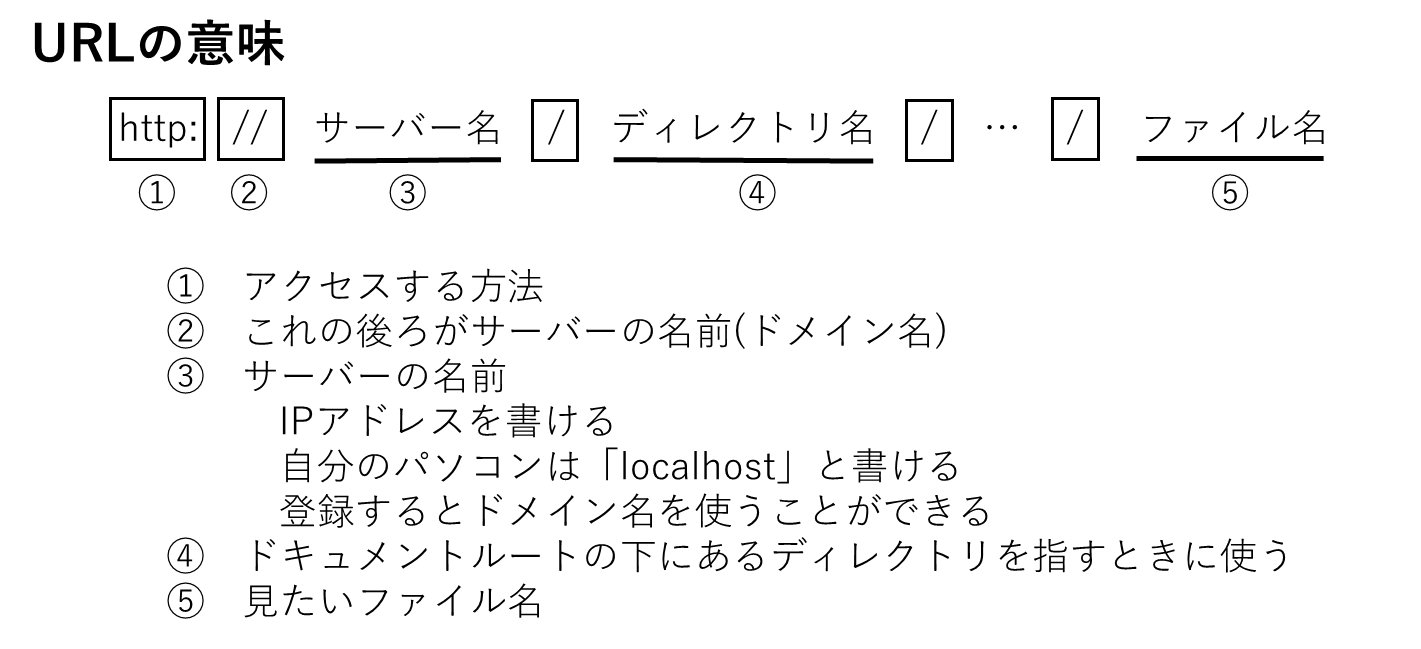
\includegraphics[width=13.894cm]{../../asset/image/ome7-img040.png}
% \flushleft

% \ \ 　\url{http://localhost:3000/}

% \ \ というURLになります。

% \ \ サーバー名の後の/（スラッシュ）はドキュメントルートを示しています。

% \ \ サーバはファイル名を指定しないとindex.htmlというファイルを開くように\ruby{設定}{せってい}されて\ \ います。

% \ \ 　\url{http://localhost:3000/}

% \ \ をブラウザのアドレスバーに打ってみましょう。

% \ \ みなさんが作ったウェブページのHTMLが表示されましたね。

% \ \ これは

% \ \ 　\url{http://localhost:3000/index.html}

% \ \ と入力しているのと同じことです。

% \bigskip

% \centering
% 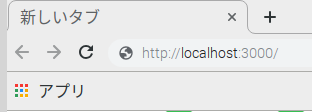
\includegraphics[width=9.551cm]{../../asset/image/ome7-img041.png}
% \flushleft


% \bigskip


% \bigskip\end{document}
